\section{Large-Scale Cosmic Filament}
\label{sec:Filament}

\begin{figure*}
    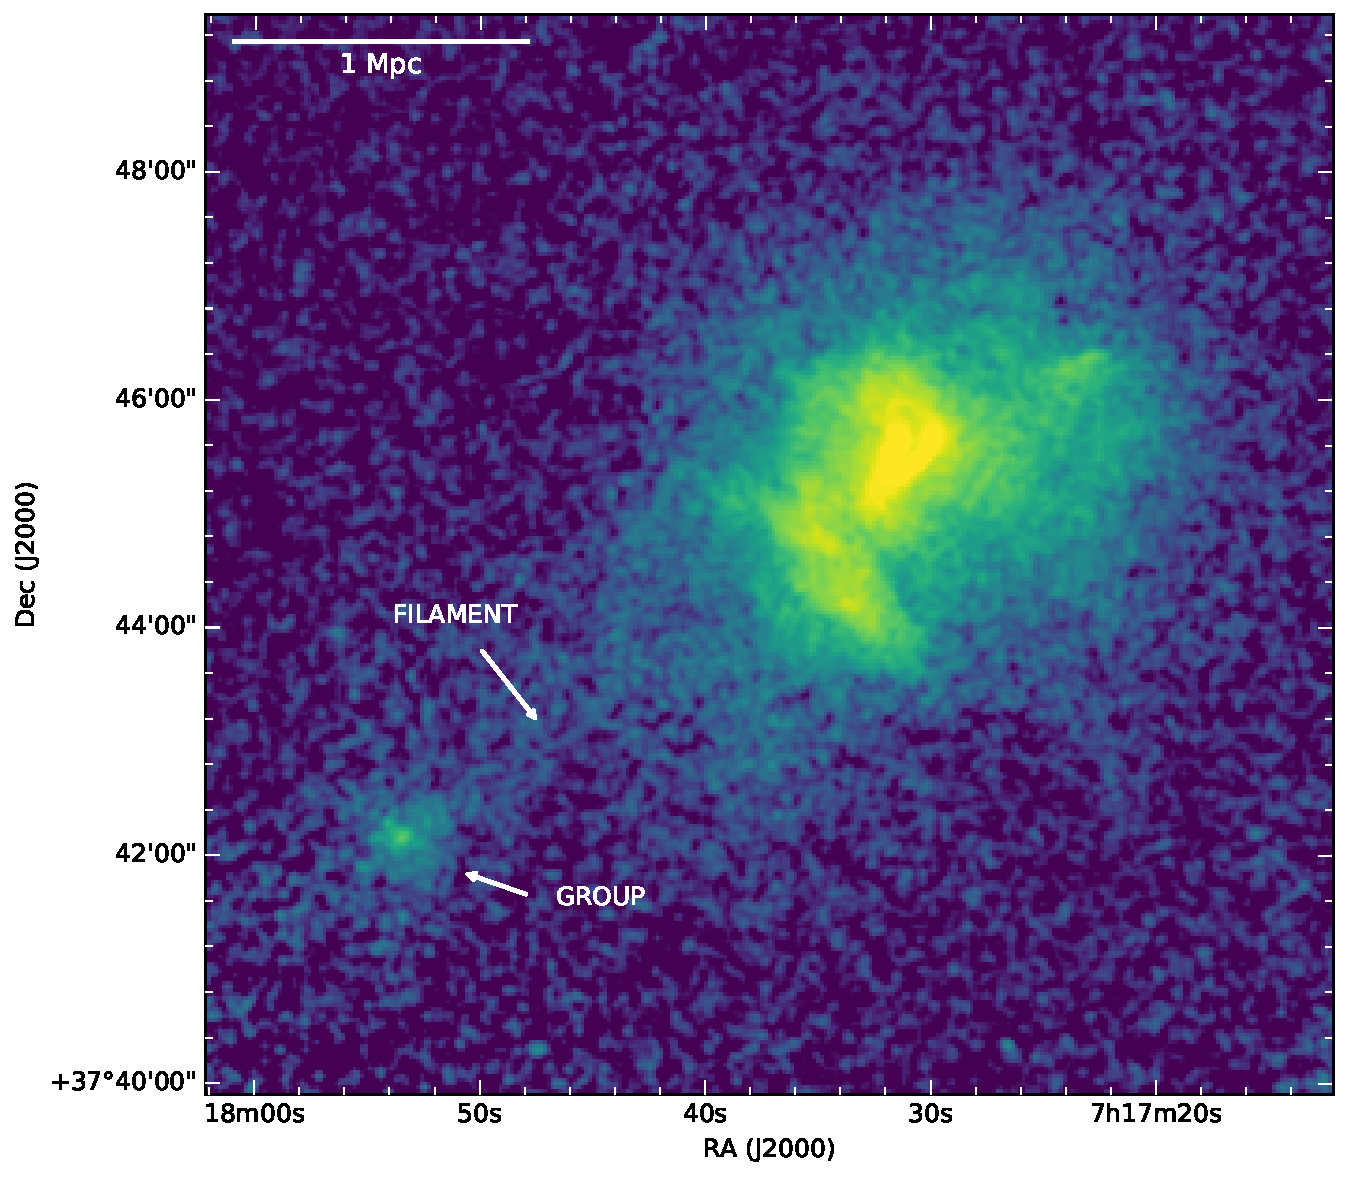
\includegraphics[width=\columnwidth]{plots/fil-labels.pdf}
    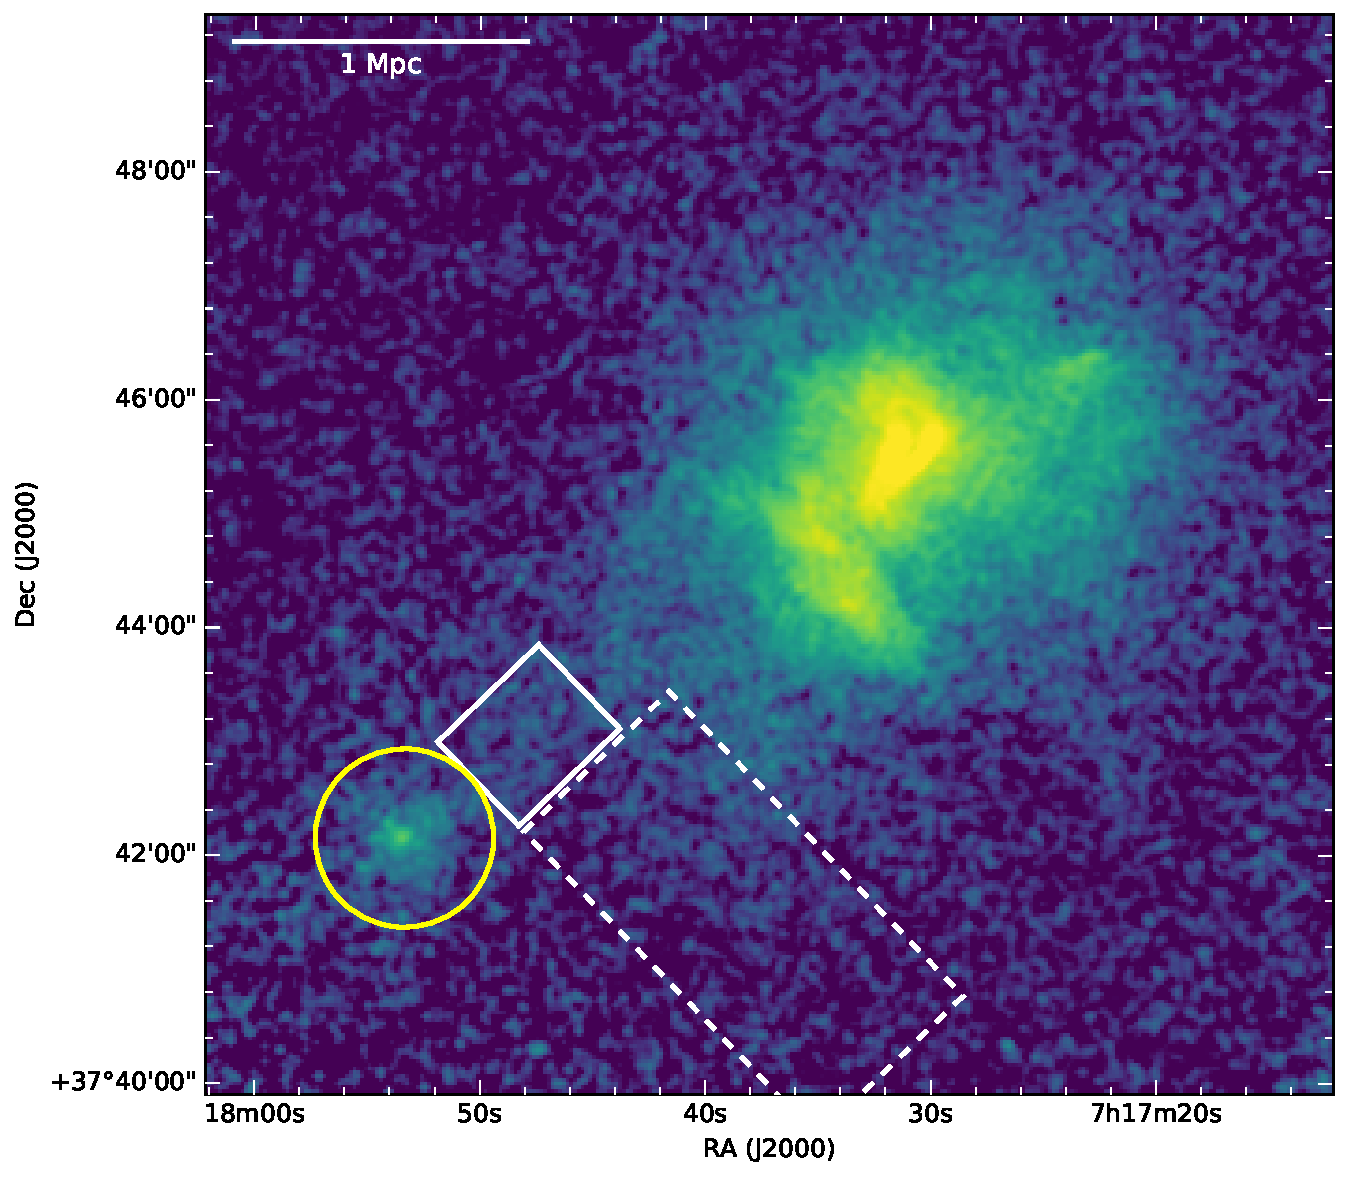
\includegraphics[width=\columnwidth]{plots/fil-regions.pdf}
    \caption{\emph{Left:} Chandra $0.5-4$~keV surface brightness map of MACS J0717.5+3745, showing the features discussed in this work. The image was exposure- and vignetting-corrected. Point sources were subtracted and the gaps were filled by sampling the regions surrounding the point sources. The gaps were filled to create a more visually appealing figure. However, the imaging analysis was done on images that did not have the gaps filled. The images used in the analysis are available online as supporting material. \emph{Right:} Regions used in the spectral analysis. The regions of main interest are drawn in solid lines, while the regions used to characterize the contaminating/surrounding emission are drawn in dashed lines. The best-fitting parameters obtained for the gas in these regions are listed in Table~\ref{tab:spectra}. \label{fig:fil}}
\end{figure*}

\begin{table}
  \caption{Parameters of the regions used for the spectral analysis. The regions are shown in Figure~\ref{fig:fil}. Uncertainties are quoted at the $\Delta C = 1$ level. \label{tab:spectra}}
  \begin{center}
    \begin{threeparttable}
      \begin{tabular}{l c c}
              \multicolumn{3}{c}{\textsc{Foreground and Background}} \\
              \hline\hline
              Model Component & Temperature\tnote{a} & Normalization\tnote{b} \\
              \hline
              Local Hot Bubble & $0.135_{-0.008}^{+0.007}$ & $7.21_{-0.18}^{+0.30} \times 10^{-7}$ \\
              Galactic Halo & $0.59_{-0.08}^{+0.09}$ & $2.78_{-0.44}^{+0.45} \times 10^{-7}$ \\
              Unresolved Background       &\multirow{2}{*}{ -- } & \multirow{2}{*}{ $4.44_{-0.37}^{+0.35} \times 10^{-7}$} \\
              Sources ObsID 16235/16305 &                                    &            \\
              Unresolved Background       &\multirow{2}{*}{ -- } & \multirow{2}{*}{ $7.02_{-0.58}^{+0.49} \times 10^{-7}$} \\
              Sources ObsID 4200               &                                    &            \\
              \multicolumn{3}{c}{} \\
              \multicolumn{3}{c}{\textsc{Large-Scale Filament}} \\
              \hline\hline
                Model Component & Temperature\tnote{a} & Normalization\tnote{b} \\
              \hline
               On Filament & $1.58_{-0.25}^{+0.51}$ & $4.00_{-0.60}^{+0.56} \times 10^{-5}$ \\
               Off Filament & $11.55_{-3.95}^{+9.09}$ & $1.55_{-0.10}^{+0.14} \times 10^{-5}$  \\
               \multicolumn{3}{c}{} \\
              \multicolumn{3}{c}{\textsc{Group in the Filament}} \\
              \hline\hline
                             & Temperature\tnote{a} & Normalization\tnote{b} \\
              \hline
                            & $3.87_{-0.51}^{+0.66}$ & $ ( 1.77\pm 0.13 ) \times 10^{-4}$ \\
              \multicolumn{3}{c}{} \\
              \multicolumn{3}{c}{\textsc{Fly-Through Core}} \\
              \hline\hline
                Model Component & Temperature\tnote{a} & Normalization\tnote{b} \\
              \hline
               Core & $6.82_{-1.36}^{+1.88}$ & $3.41_{-0.25}^{+0.29} \times 10^{-4}$ \\
               N+S of Core & $7.47_{-0.86}^{+1.11}$ & $2.08_{-0.78}^{+0.77} \times 10^{-4}$  \\
               Ahead of Core & $5.06_{-0.98}^{+1.61}$ & $8.52_{-0.77}^{+0.88} \times 10^{-5}$  \\
               Behind Core & $10.89_{-1.27}^{+2.05}$ & $3.92_{-0.09}^{+0.10} \times 10^{-4}$  \\
      \end{tabular}
      \begin{tablenotes}
              \item[a] Units of keV.
              \item[b] Units of cm$^{-5}$~arcmin$^{-2}$ for the thermal components, and photons~keV$^{-1}$~cm$^{-2}$~s$^{-1}$~arcmin$^{-2}$ at 1~keV for the power-law components.
      \end{tablenotes}
    \end{threeparttable}
  \end{center}
\end{table}

To define the region of the filament that is least contaminated by ICM emission, we examined the surface brightness profile in a rectangular region aligned with the filament. In this region, the surface brightness decreases away from the cluster center, and then increases again when the region intersects the SE group located along the filament; there is no radial range in this region where the surface brightness is flat. This suggests that the ICM of MACS~J0717.5+3745 contaminates the filament, and this contamination needs to be considered when modeling the filament emission.

To model the filament and the contamination from the ICM, we extracted spectra in three rectangular regions: one centered on the filament, and two positioned to the W and to the E of it. These regions are shown in Figure~\ref{fig:fil}. The regions were chosen to avoid the bright parts of the ICM, as well as emission from the SE galaxy group. The emission in the W and E regions was modeled with a single thermal component, while the emission in the filament region was modeled with two thermal components--one describing ICM contamination, whose parameters were linked to those of the thermal component used to describe the W and E regions, and one describing emission from the filament. The spectra from the three regions were fitted simultaneously. Table~\ref{tab:spectra} lists the best-fitting parameters obtained for a gas metallicity of 0.2 solar. Varying the metallicity causes only minor changes to the best-fitting parameters, well within the statistical uncertainty ranges. In the \textsc{Jupyter} notebook supporting this letter, we also show the results obtained for metallicities of 0 and 0.1 solar.

The \textsc{XSpec} normalizations of the thermal components listed in Table~\ref{tab:spectra} are defined as:
\begin{equation}
	\mathcal{N} = \frac{n_{\rm e} \, n_{\rm H} \, V}{10^{14} \, \pi \, S_{\rm reg} \, D_{\rm A}^2 \, (1+z)^2} \, , \nonumber
\end{equation}
if we assume the density to be constant in each region, where $n_{\rm e}$ is the electron number density, $n_{\rm H}$ is the hydrogen number density, $V$ is the volume of the region, $S_{\rm reg}$ is the projected area of the region, $D_{\rm A}$ is the angular size distance to the cluster, and $z$ is the cluster redshift.

To calculate the density of the filament in the region shown in Figure~\ref{fig:fil}, we assumed this region has an elliptic cylinder geometry. \citet{Jauzac2012} determined that the filament is inclined at 75 degrees with respect to the plane of the sky, and has a diameter of $\sim 1.6$~Mpc and a length of $\sim 19$~Mpc. Therefore, we assumed the region from which we extracted the spectrum of the filament to be an elliptic cylinder with a length:
\begin{equation}
	L = \frac{l_{\rm box}}{\cos{75^{\circ}}} \sim 2.2 \; {\rm Mpc}\, 
\end{equation}
where $l_{\rm box}$ is the length of the box region in Figure~\ref{fig:fil}, and a base with major axis $a = 0.8$~Mpc and a minor axis equal to the length of the box in Figure~\ref{fig:fil}, i.e. $b = 0.2$~Mpc. The volume of this region is $V = \pi a\, b \, L = 1.1$~Mpc$^3$. We further assumed that $n_{\rm H} = 1.2 \, n_{\rm e}$ \citep{Bohringer2010}. The area of the filament region shown in Figure~\ref{fig:fil} is $1.4$~arcmin$^2$. Therefore, for an \textsc{XSpec} normalization of $\sim 4\times 10^{-5}$~cm$^{-5}$~arcmin${^{-2}}$ (Table~\ref{tab:spectra}), the electron number density is $\sim 1\times 10^{-4}$~cm$^{-3}$. Assuming a baryon fraction of 0.044 \citep{Kirkman2003}, the filament is over-dense by a factor of $\sim 250$ compared to the mean baryon density of the Universe. Our result is consistent with that of \citet{Jauzac2012}, who used lensing data to calculate a filament over-density factor of $206 \pm 46$. Our result is also consistent with the upper range over-densities predicted from numerical simulations of cosmic filaments \citep[e.g.,][]{Gheller2015}.

For a baryon fraction of 0.15 \citep{Mantz2014}, the density of the filament is equivalent to a mass of $\sim 2\times 10^{13}$~M$_{\odot}$~Mpc$^{-3}$.  Approximating the geometry of the full filament as a cylinder with a length of $19$~Mpc and a diameter of $1.6$~Mpc, our result implies a total filament mass of $\sim 7\times 10^{14}$~M$_\odot$. The gas density is expected to decrease with increasing distance from the cluster center. Therefore, our mass estimate should only be interpreted as an upper limit on the total mass of the filament.





